% uid: ""
% school: "college"
% level: "7eme"
% chapter: "التناظر المحوري"
% chapter_slug: "symetrie-axiale"
% title: "صحيح أم خاطئ ؟"
% difficulty: "Facile"
% tags: ["vrai-faux", "symetrie-axiale", "contre-exemple", "proprietes"]
% provenance: "own"
% batch: "2026-11-27-symetrie-axiale-7eme"
% Exercice 3/10 de la série 7ème « التناظر المحوري » (statement + \axsol + solution). Compiler avec XeLaTeX + axiomath.sty (+ axiomaths-logo.png).
\documentclass[12pt,a4paper]{article}
\usepackage[level=7b,color=0F766E]{axiomath}
\newcommand{\cm}{\,\mathrm{cm}}
\axsetup{title={التناظر المحوري}, corrige}

\begin{document}

\begin{corr}[title={صحيح أم خاطئ ؟}, stars=1, source={Axiomaths}]
حدّد إن كانت كل عبارة صحيحة أم خاطئة، ثم علّل إجابتك. $\Delta$ مستقيم.
\begin{enumerate}
  \item مناظرة نقطة بالنسبة إلى $\Delta$ تنتمي دائما إلى $\Delta$.
  \item إذا كانت $B$ مناظرة $A$ بالنسبة إلى $\Delta$ فإن $A$ مناظرة $B$ بالنسبة إلى $\Delta$.
  \item النقاط $A$ و $B$ و $C$ على استقامة واحدة، إذن مناظراتها بالنسبة إلى $\Delta$ على استقامة واحدة.
  \item مناظر مستقيم $d$ بالنسبة إلى $\Delta$ هو دائما مستقيم موازٍ لـ $d$.
  \item للدائرة محور تناظر واحد.
\end{enumerate}
\axsol
\begin{enumerate}[itemsep=12pt]
  \item \textbf{خاطئ.} فقط نقاط $\Delta$ هي مناظرة نفسها. إذا كانت $A$ خارج $\Delta$ فإن $A'$ في الجهة الأخرى من $\Delta$.
  \item \textbf{صحيح.} $\Delta$ محور القطعة $[AB]$ ، وهي نفسها القطعة $[BA]$.
  \item \textbf{صحيح.}
  \begin{prop}[الحفاظ على الاستقامة]
  التناظر المحوري يحافظ على \ib{الاستقامة}.
  \end{prop}
  \item \textbf{خاطئ.} مثال مضاد : $d$ يقطع $\Delta$ في نقطة $I$ ولا يعامده. مناظر $I$ هو $I$ ، فالمستقيم $d'$ يمرّ أيضا من $I$. إذن $d$ و $d'$ يتقاطعان في $I$ : ليسا متوازيين.
  \begin{center}
  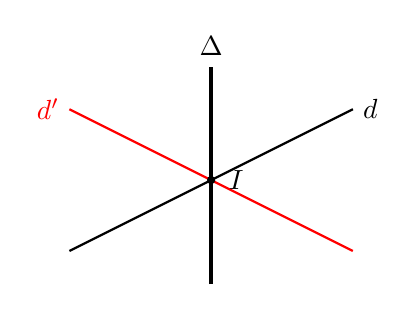
\begin{tikzpicture}[scale=0.6]
    \draw[very thick] (0,-2.2)--(0,2.4) node[above] {$\Delta$};
    \draw[thick] (-3,-1.5)--(3,1.5) node[right] {$d$};
    \draw[thick,red] (3,-1.5)--(-3,1.5) node[left] {$d'$};
    \fill (0,0) circle (2.5pt) node[right=3pt] {$I$};
  \end{tikzpicture}
  \end{center}
  \item \textbf{خاطئ.} كل مستقيم يمرّ من مركز الدائرة هو محور تناظر لها : للدائرة \ib{عدد لا نهائي من محاور التناظر}.
\end{enumerate}
\end{corr}

\end{document}
